\documentclass[12pt, spanish]{article}
\usepackage[spanish]{babel}
\selectlanguage{spanish}
\usepackage{natbib}
\usepackage{url}
\usepackage[utf8x]{inputenc}
\usepackage{graphicx}
\graphicspath{{images/}}
\usepackage{array}
\usepackage{longtable}
\usepackage{parskip}
\usepackage{fancyhdr}
\usepackage{vmargin}
\usepackage{listings}
\usepackage{adjustbox}
\usepackage{pdflscape}
\usepackage[shortlabels]{enumitem}

\setlist[enumerate]{
labelsep=8pt,
labelindent=0.3\parindent,
itemindent=0pt,
leftmargin=*,
before=\setlength{\listparindent}{-\leftmargin},
}

\usepackage[default]{sourcesanspro}

\setmarginsrb{2 cm}{1 cm}{2 cm}{2 cm}{1 cm}{1.5 cm}{1 cm}{1.5 cm}

\title{Fundamentos de Ingeniería del Software:\\
Práctica 4  \hspace{0.05cm} }
\date{}
\author{
\begin{center}
Martina Álvarez Lorenzo  \\
Pablo Ariza García  \\
David Gutiérrez Pérez  \\
Yeray López Ramírez \\
\end{center}
}

\renewcommand*\contentsname{hola}

\makeatletter
\let\thetitle\@title
\let\theauthor\@author
\let\thedate\@date
\makeatother

\pagestyle{fancy}
\fancyhf{}
\rhead{}
\chead{\thedate}
\lhead{\thetitle}
\cfoot{\thepage}

\begin{document}
%%%%%%%%%%%%%%%%%%%%%%%%%%%%%%%%%%%%%%%%%%%%%%%%%%%%%%%%%%%%%%%%%%%%%%%%%%%%%%%%%%%%%%%%%

\begin{titlepage}
  \centering
  \vspace*{0.5 cm}
  
\includegraphics[scale = 0.20]{logoUGR.png}\\[1.0 cm]
  \textsc{\LARGE Universidad de Granada}\\[2.0 cm]
  \textsc{\large 2ºD}\\[0.5 cm]
  \textsc{\large Grado en Ingeniería Informática}\\[0.5 cm]              
  \rule{\linewidth}{0.2 mm} \\[0.4 cm]
  { \huge \bfseries \thetitle}\\
  \rule{\linewidth}{0.2 mm} \\[1.5 cm]
  
      
  \theauthor

  \vfill
  
\end{titlepage}

\newpage

%%%%%%%%%%%%%%%%%%%%%%%%%%%%%%%%%%%%%%%%%%%%%%%%%%%%%%%%%%%%%%%%%%%%%%%%%%%%%%%%%%%%%%%%%


\tableofcontents
\pagebreak

\section{Diagramas de Comunicación}

\begin{enumerate}
 \item (2 puntos) Resolver la ecuación en recurrencias ${T(n) = 3T(n/3) + log_3(n)}$ , indicando el orden resultante asumiendo que la ecuación se obtuvo para el caso peor de un algoritmo.
\end{enumerate}
\subsection{Diagramas de Martina Álvarez Lorenzo}
\begin{centering}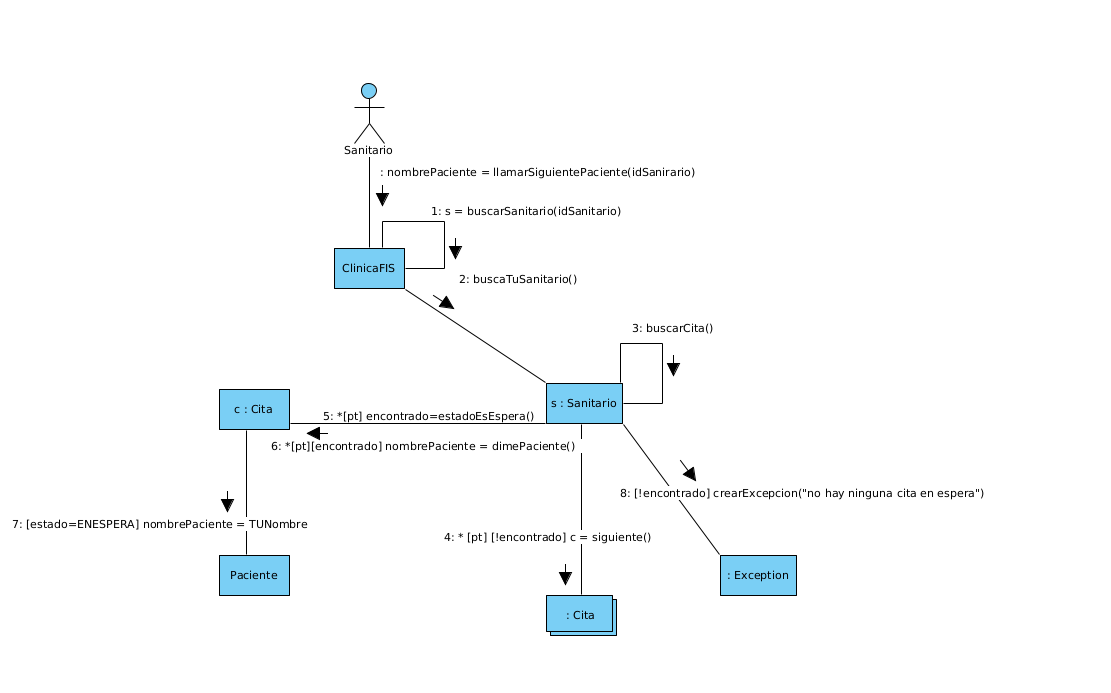
\includegraphics[scale = 0.40]{C1.png}\\[1.0 cm]\end{centering}
\begin{centering}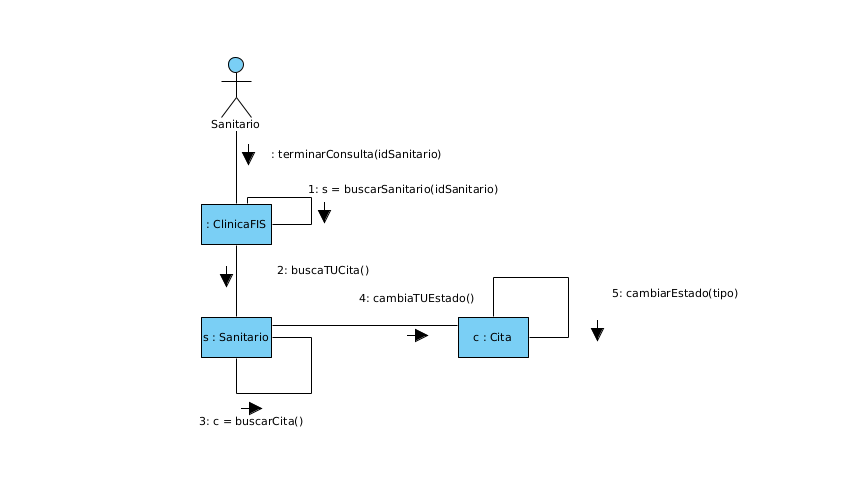
\includegraphics[scale = 0.50]{C2.png}\\[1.0 cm]\end{centering}
\begin{centering}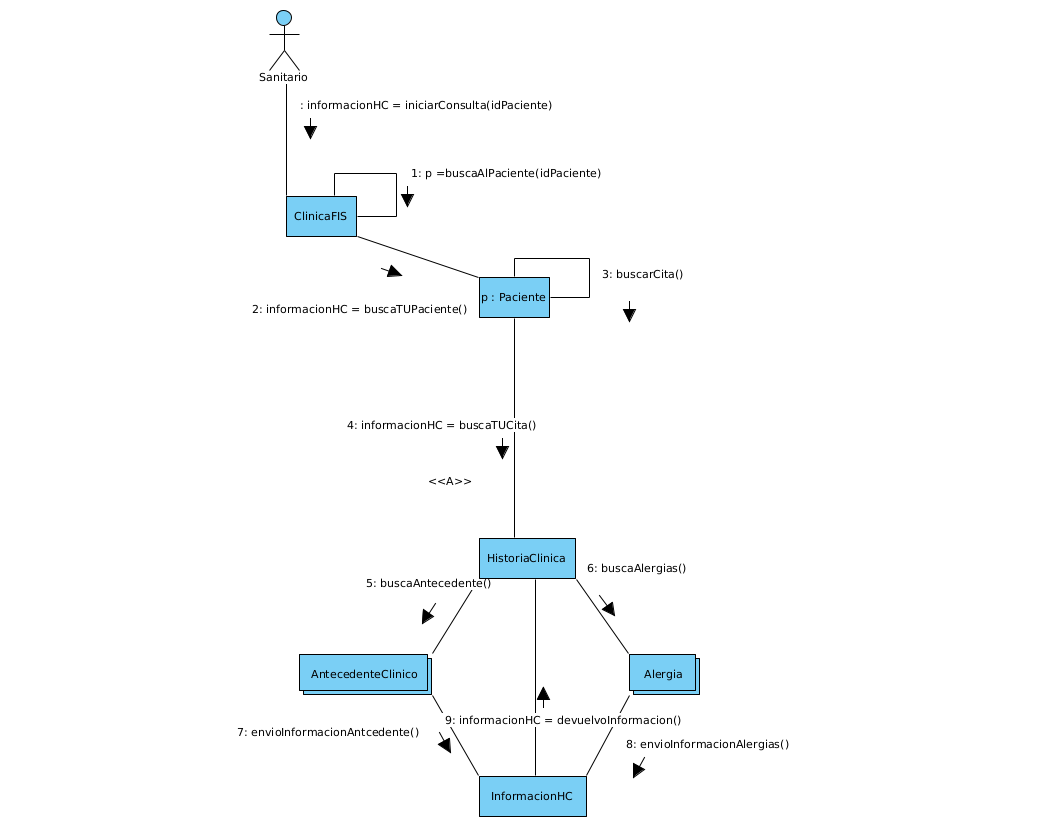
\includegraphics[scale = 0.45]{C3.png}\\[1.0 cm]\end{centering}
\begin{centering}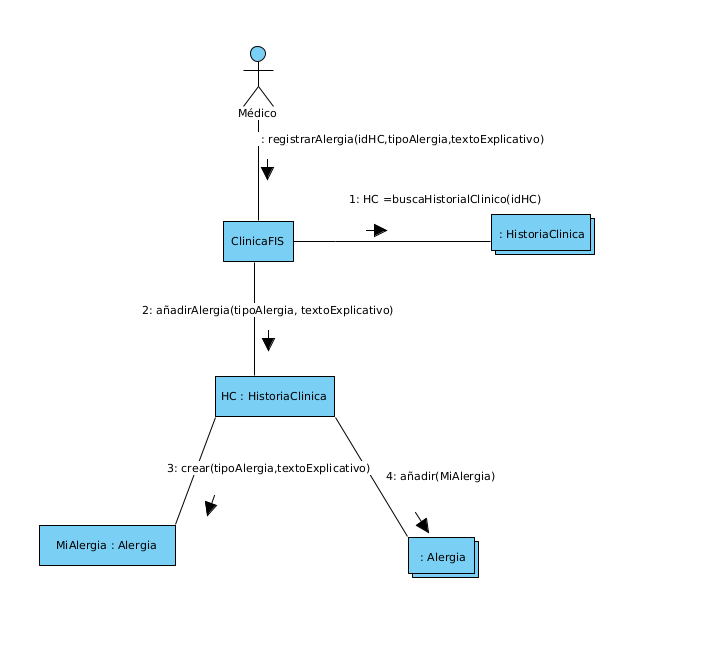
\includegraphics[scale = 0.50]{C4.png}\\[1.0 cm]\end{centering} %boooooooooooooooomb
\begin{centering}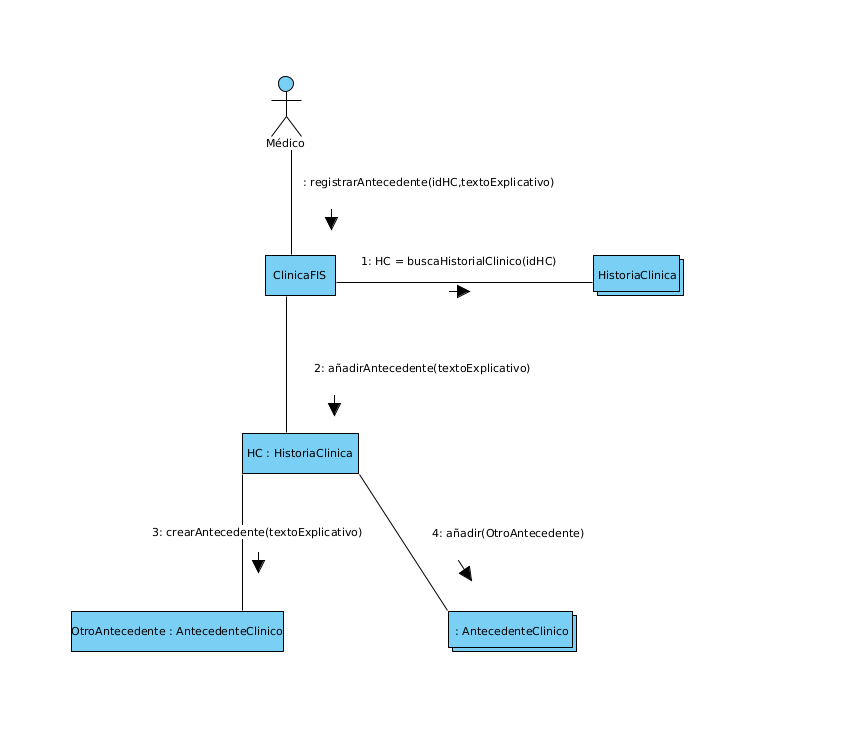
\includegraphics[scale = 0.50]{C5.png}\\[1.0 cm]\end{centering}

\pagebreak

\subsection{Diagramas de David Gutiérrez Pérez}
\begin{centering}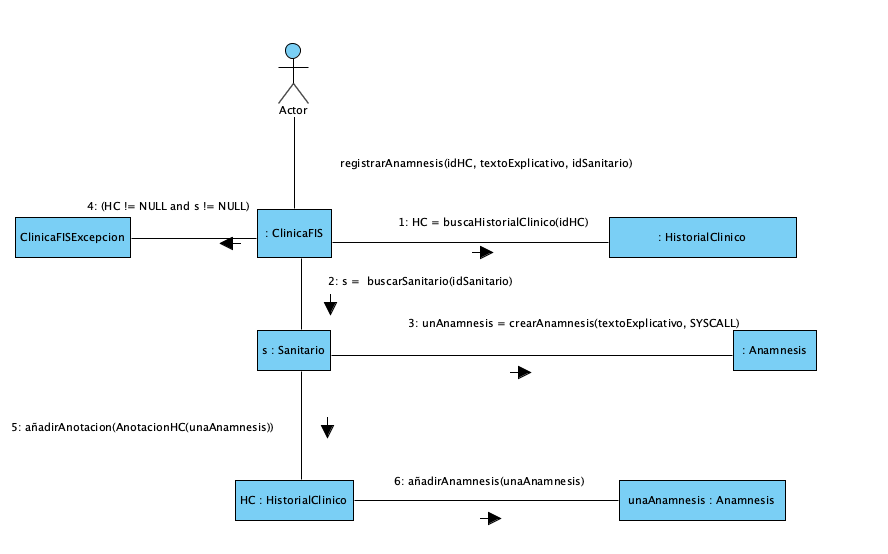
\includegraphics[scale = 0.50]{C6.png}\\[1.0 cm]\end{centering}
\begin{centering}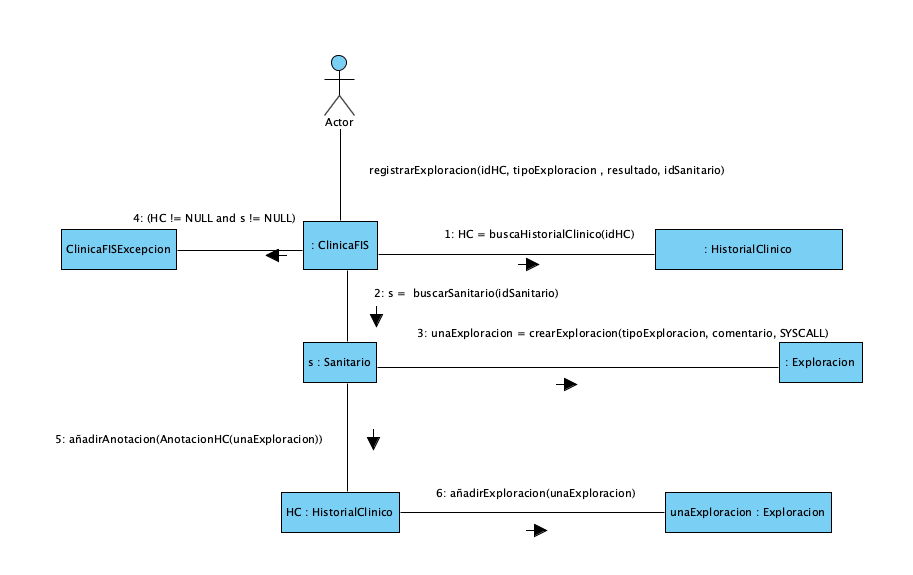
\includegraphics[scale = 0.50]{C7.png}\\[1.0 cm]\end{centering}
\begin{centering}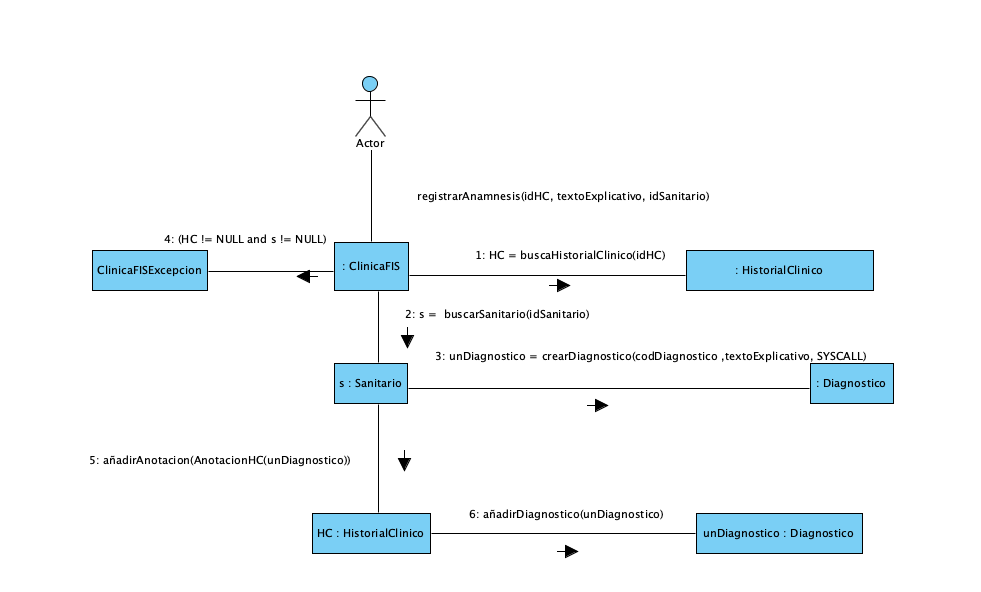
\includegraphics[scale = 0.45]{C8.png}\\[1.0 cm]\end{centering}
\begin{centering}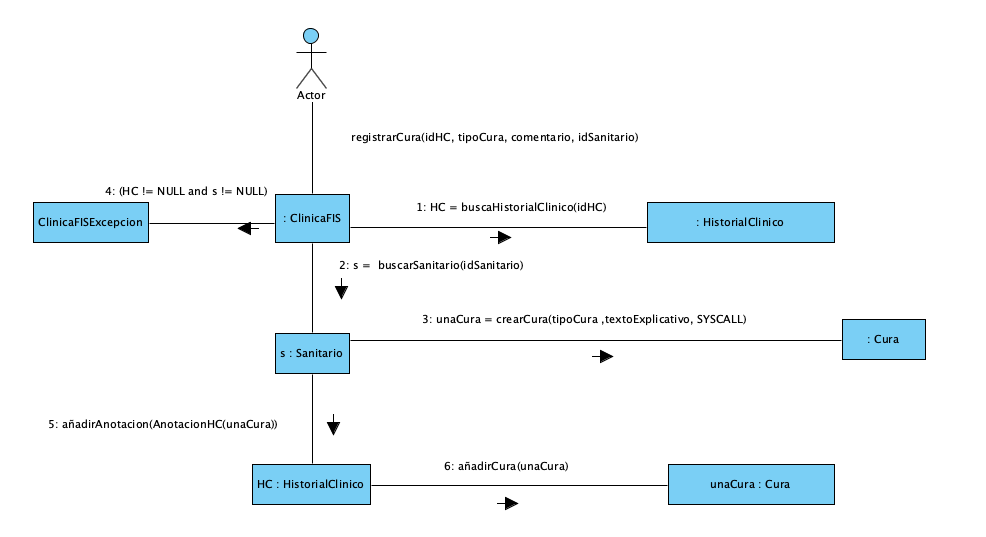
\includegraphics[scale = 0.45]{C9.png}\\[1.0 cm]\end{centering}
\begin{centering}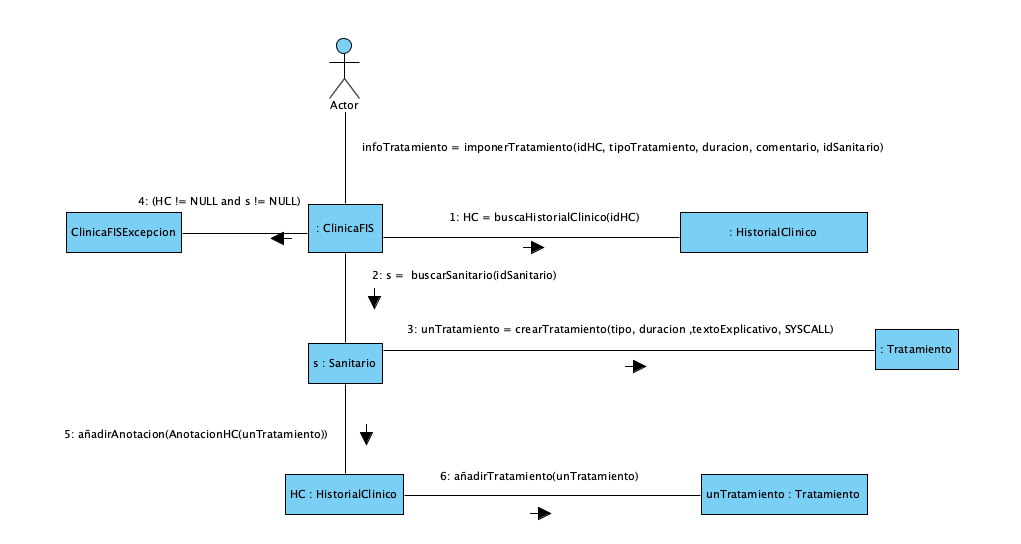
\includegraphics[scale = 0.45]{C10.png}\\[1.0 cm]\end{centering}

\pagebreak

\subsection{Diagramas de Pablo Ariza García}
\begin{centering}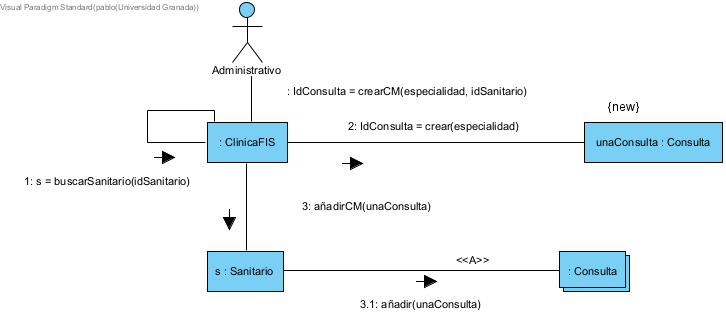
\includegraphics[scale = 0.50]{C11.png}\\[1.0 cm]\end{centering}
\begin{centering}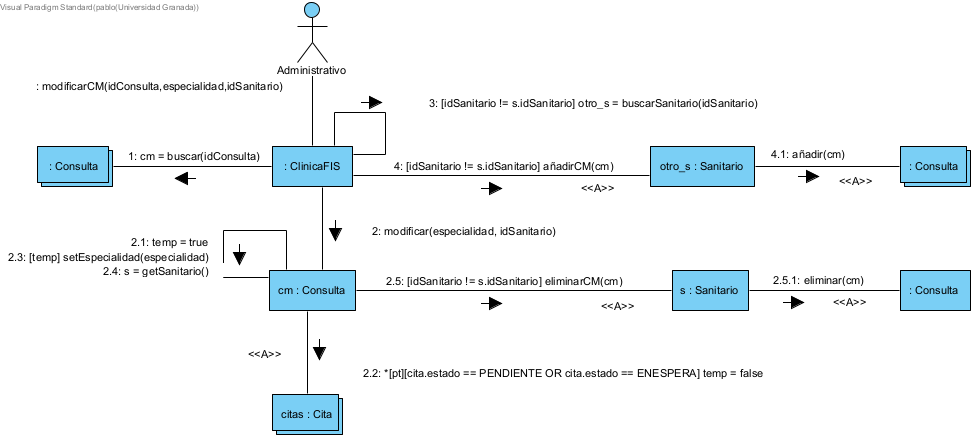
\includegraphics[scale = 0.50]{C12.png}\\[1.0 cm]\end{centering}
\begin{centering}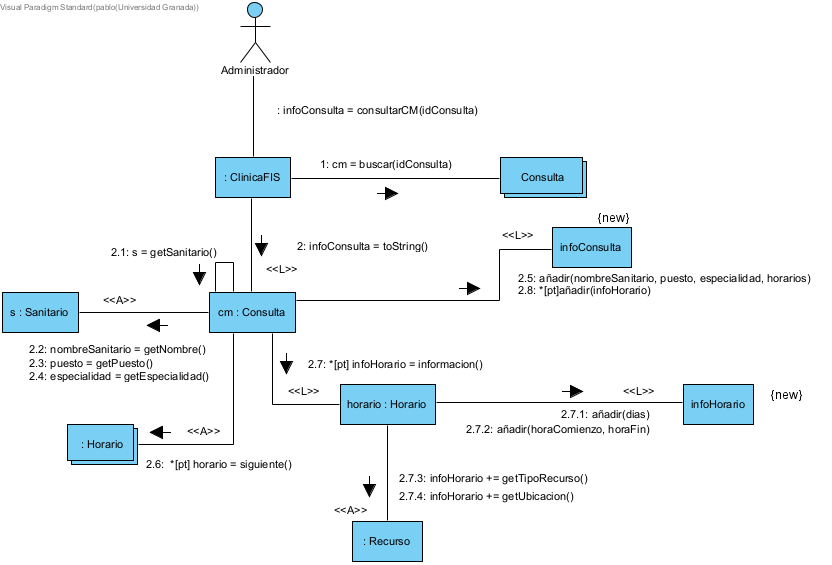
\includegraphics[scale = 0.50]{C13.png}\\[1.0 cm]\end{centering}
\begin{centering}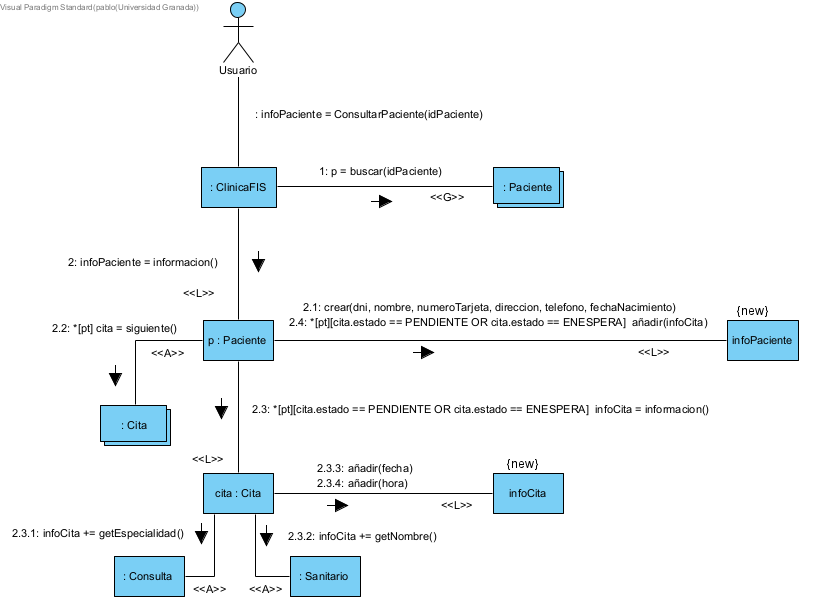
\includegraphics[scale = 0.50]{C14.png}\\[1.0 cm]\end{centering}
\begin{centering}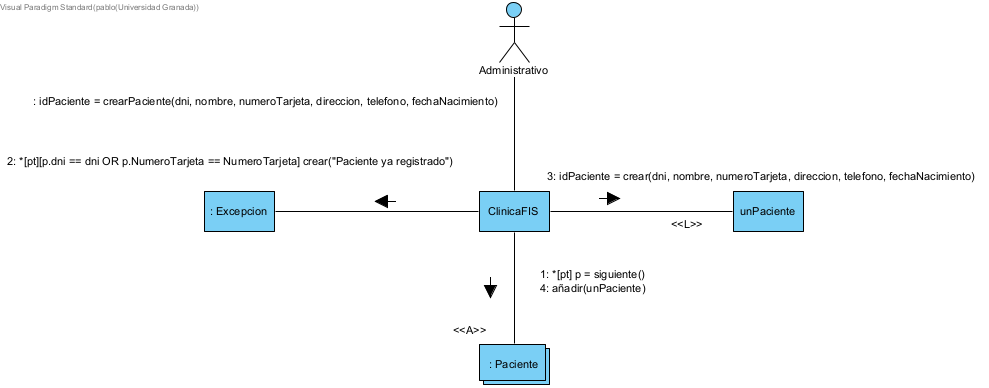
\includegraphics[scale = 0.50]{C15.png}\\[1.0 cm]\end{centering}

\pagebreak

\subsection{Diagramas de Yeray López Ramírez}
\begin{centering}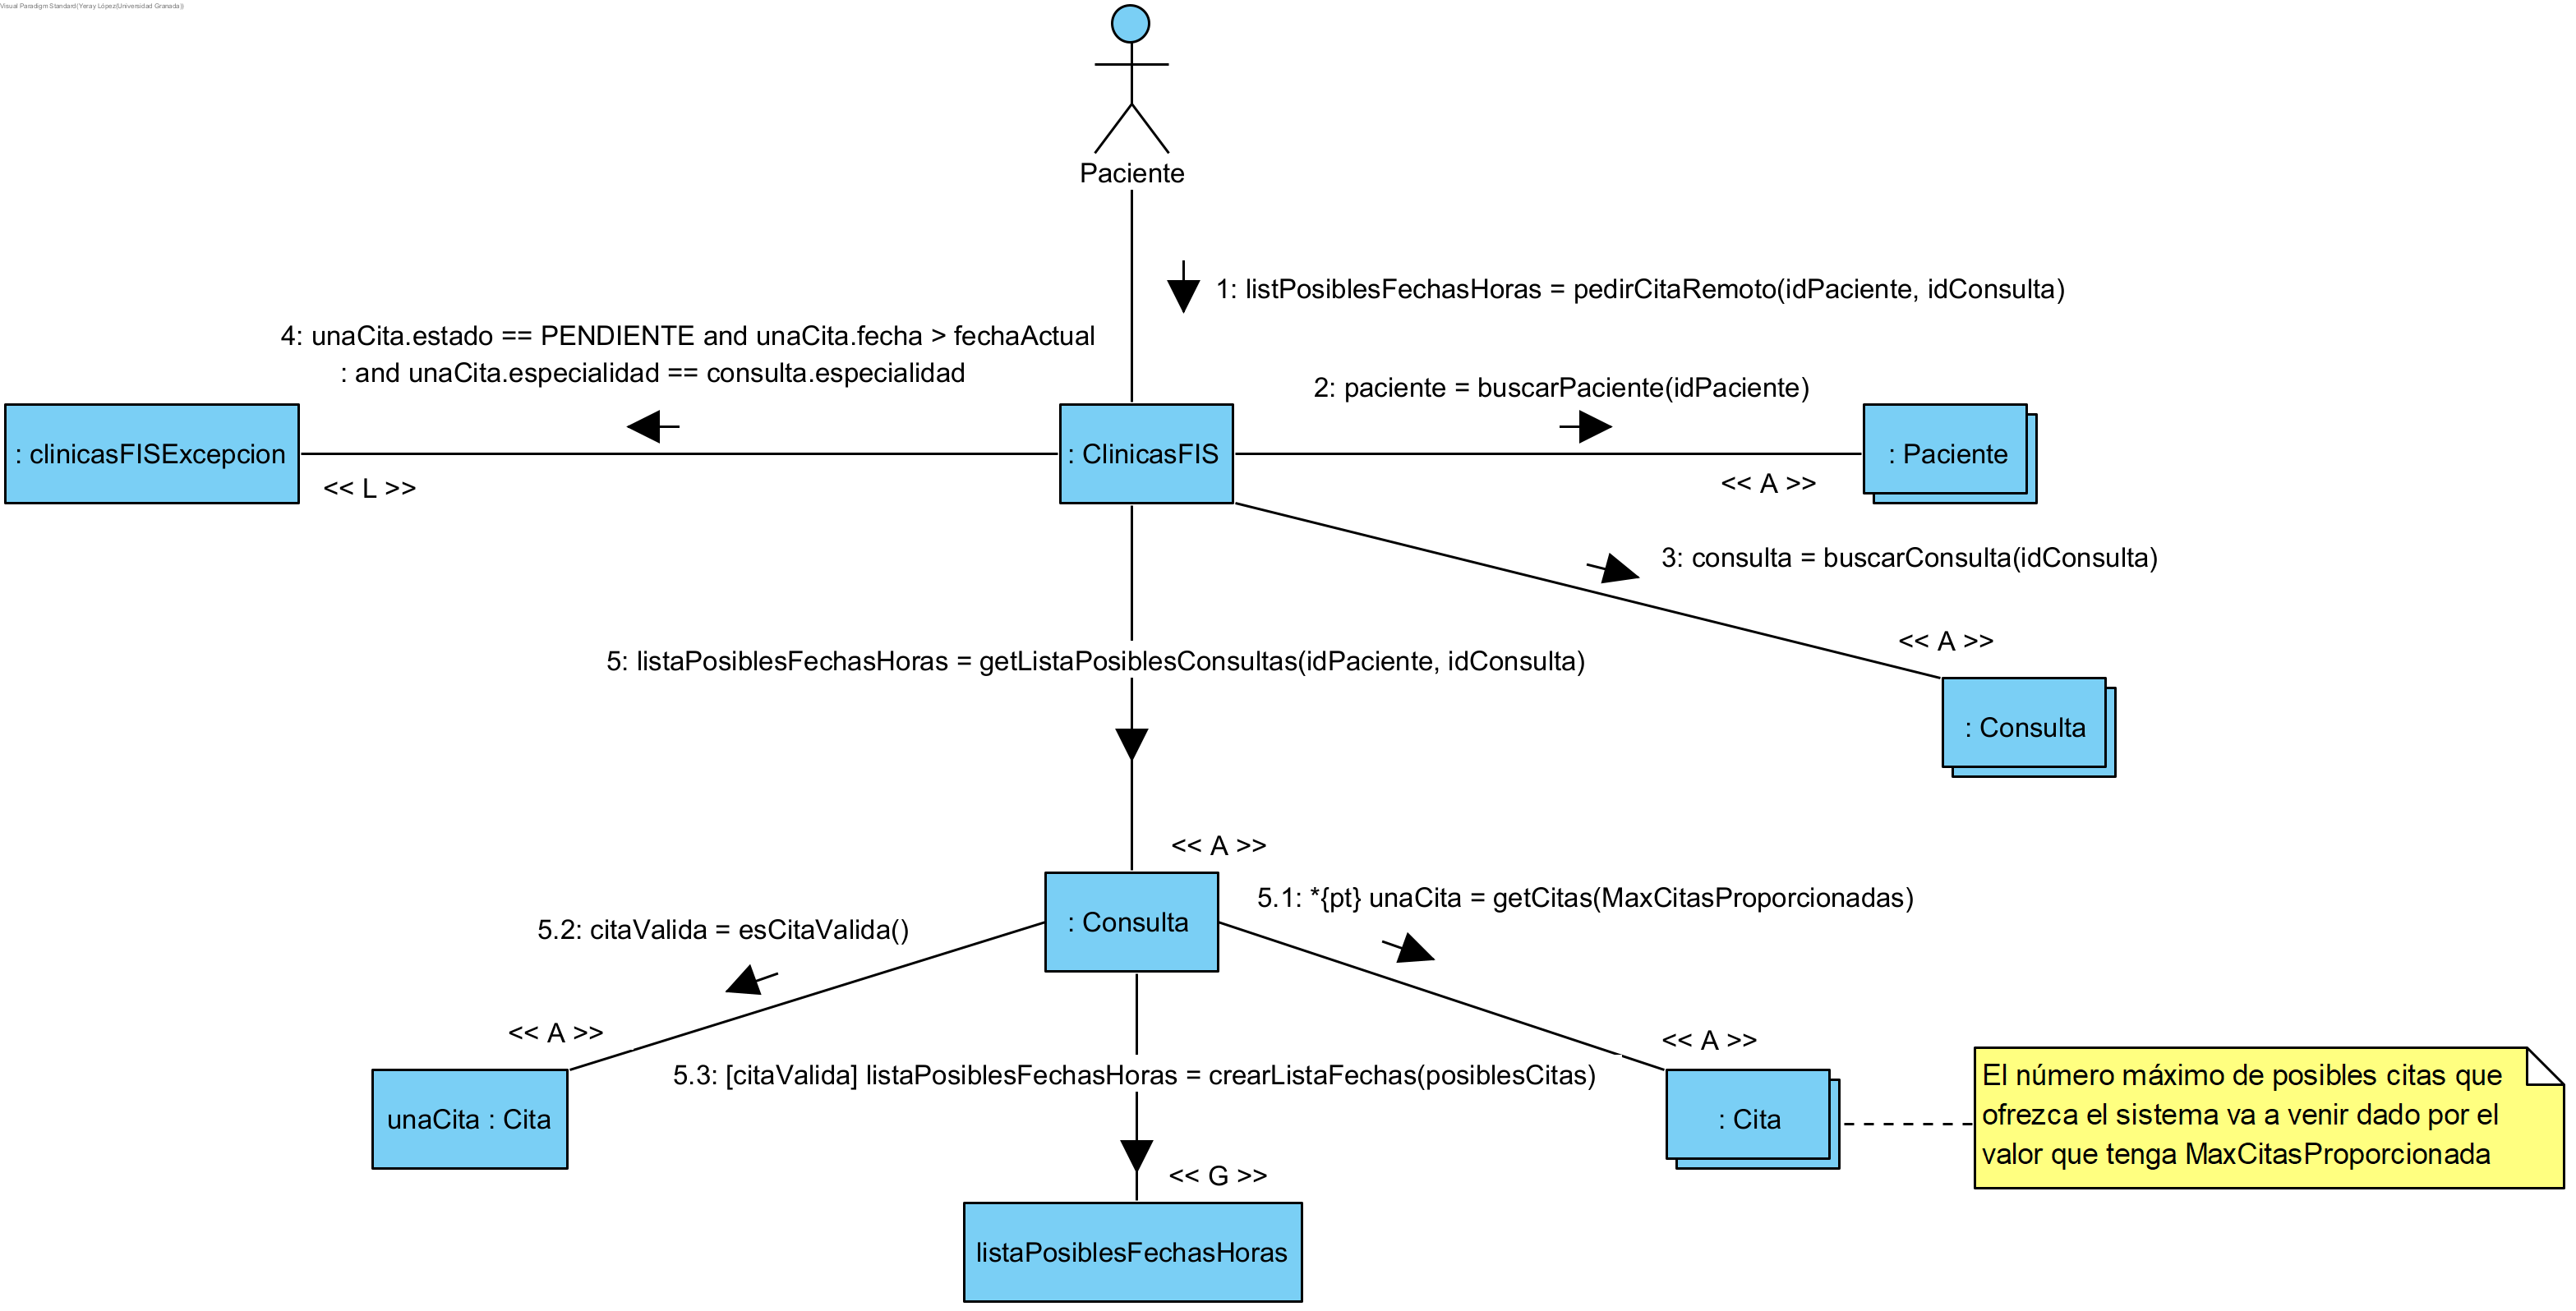
\includegraphics[scale = 0.45]{C16.png}\\[1.0 cm]\end{centering}
\begin{centering}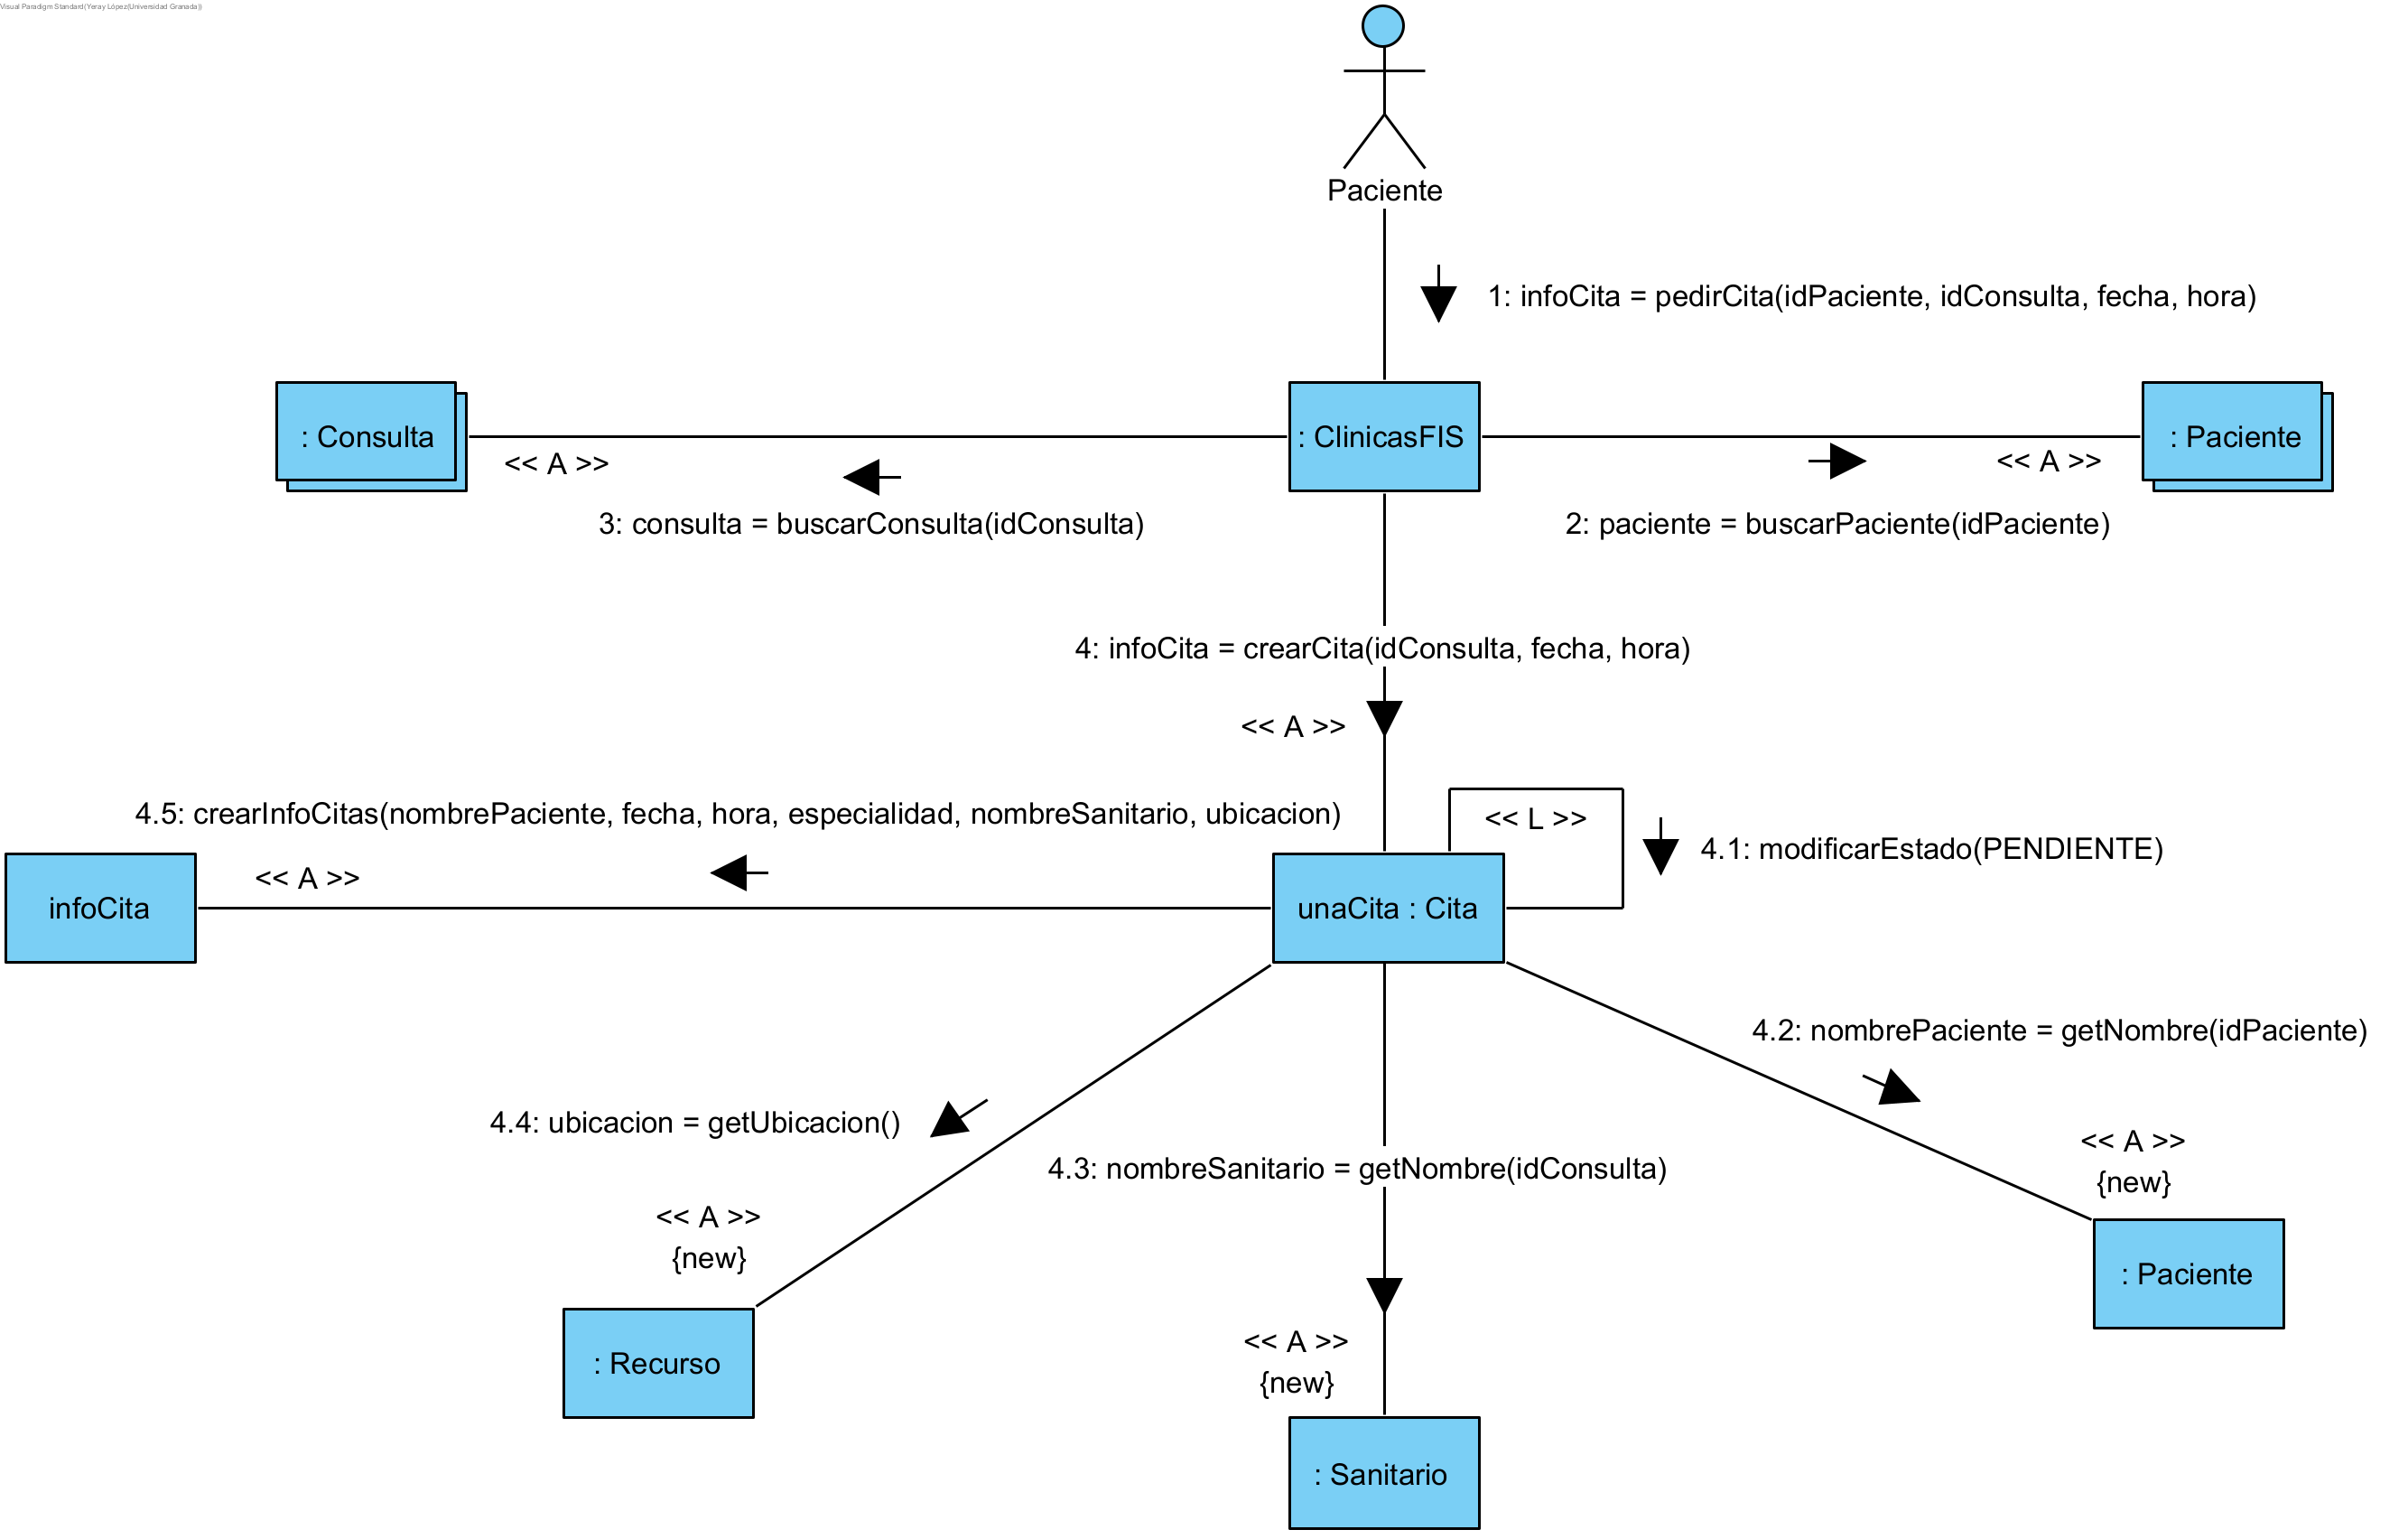
\includegraphics[scale = 0.50]{C17.png}\\[1.0 cm]\end{centering}
\begin{centering}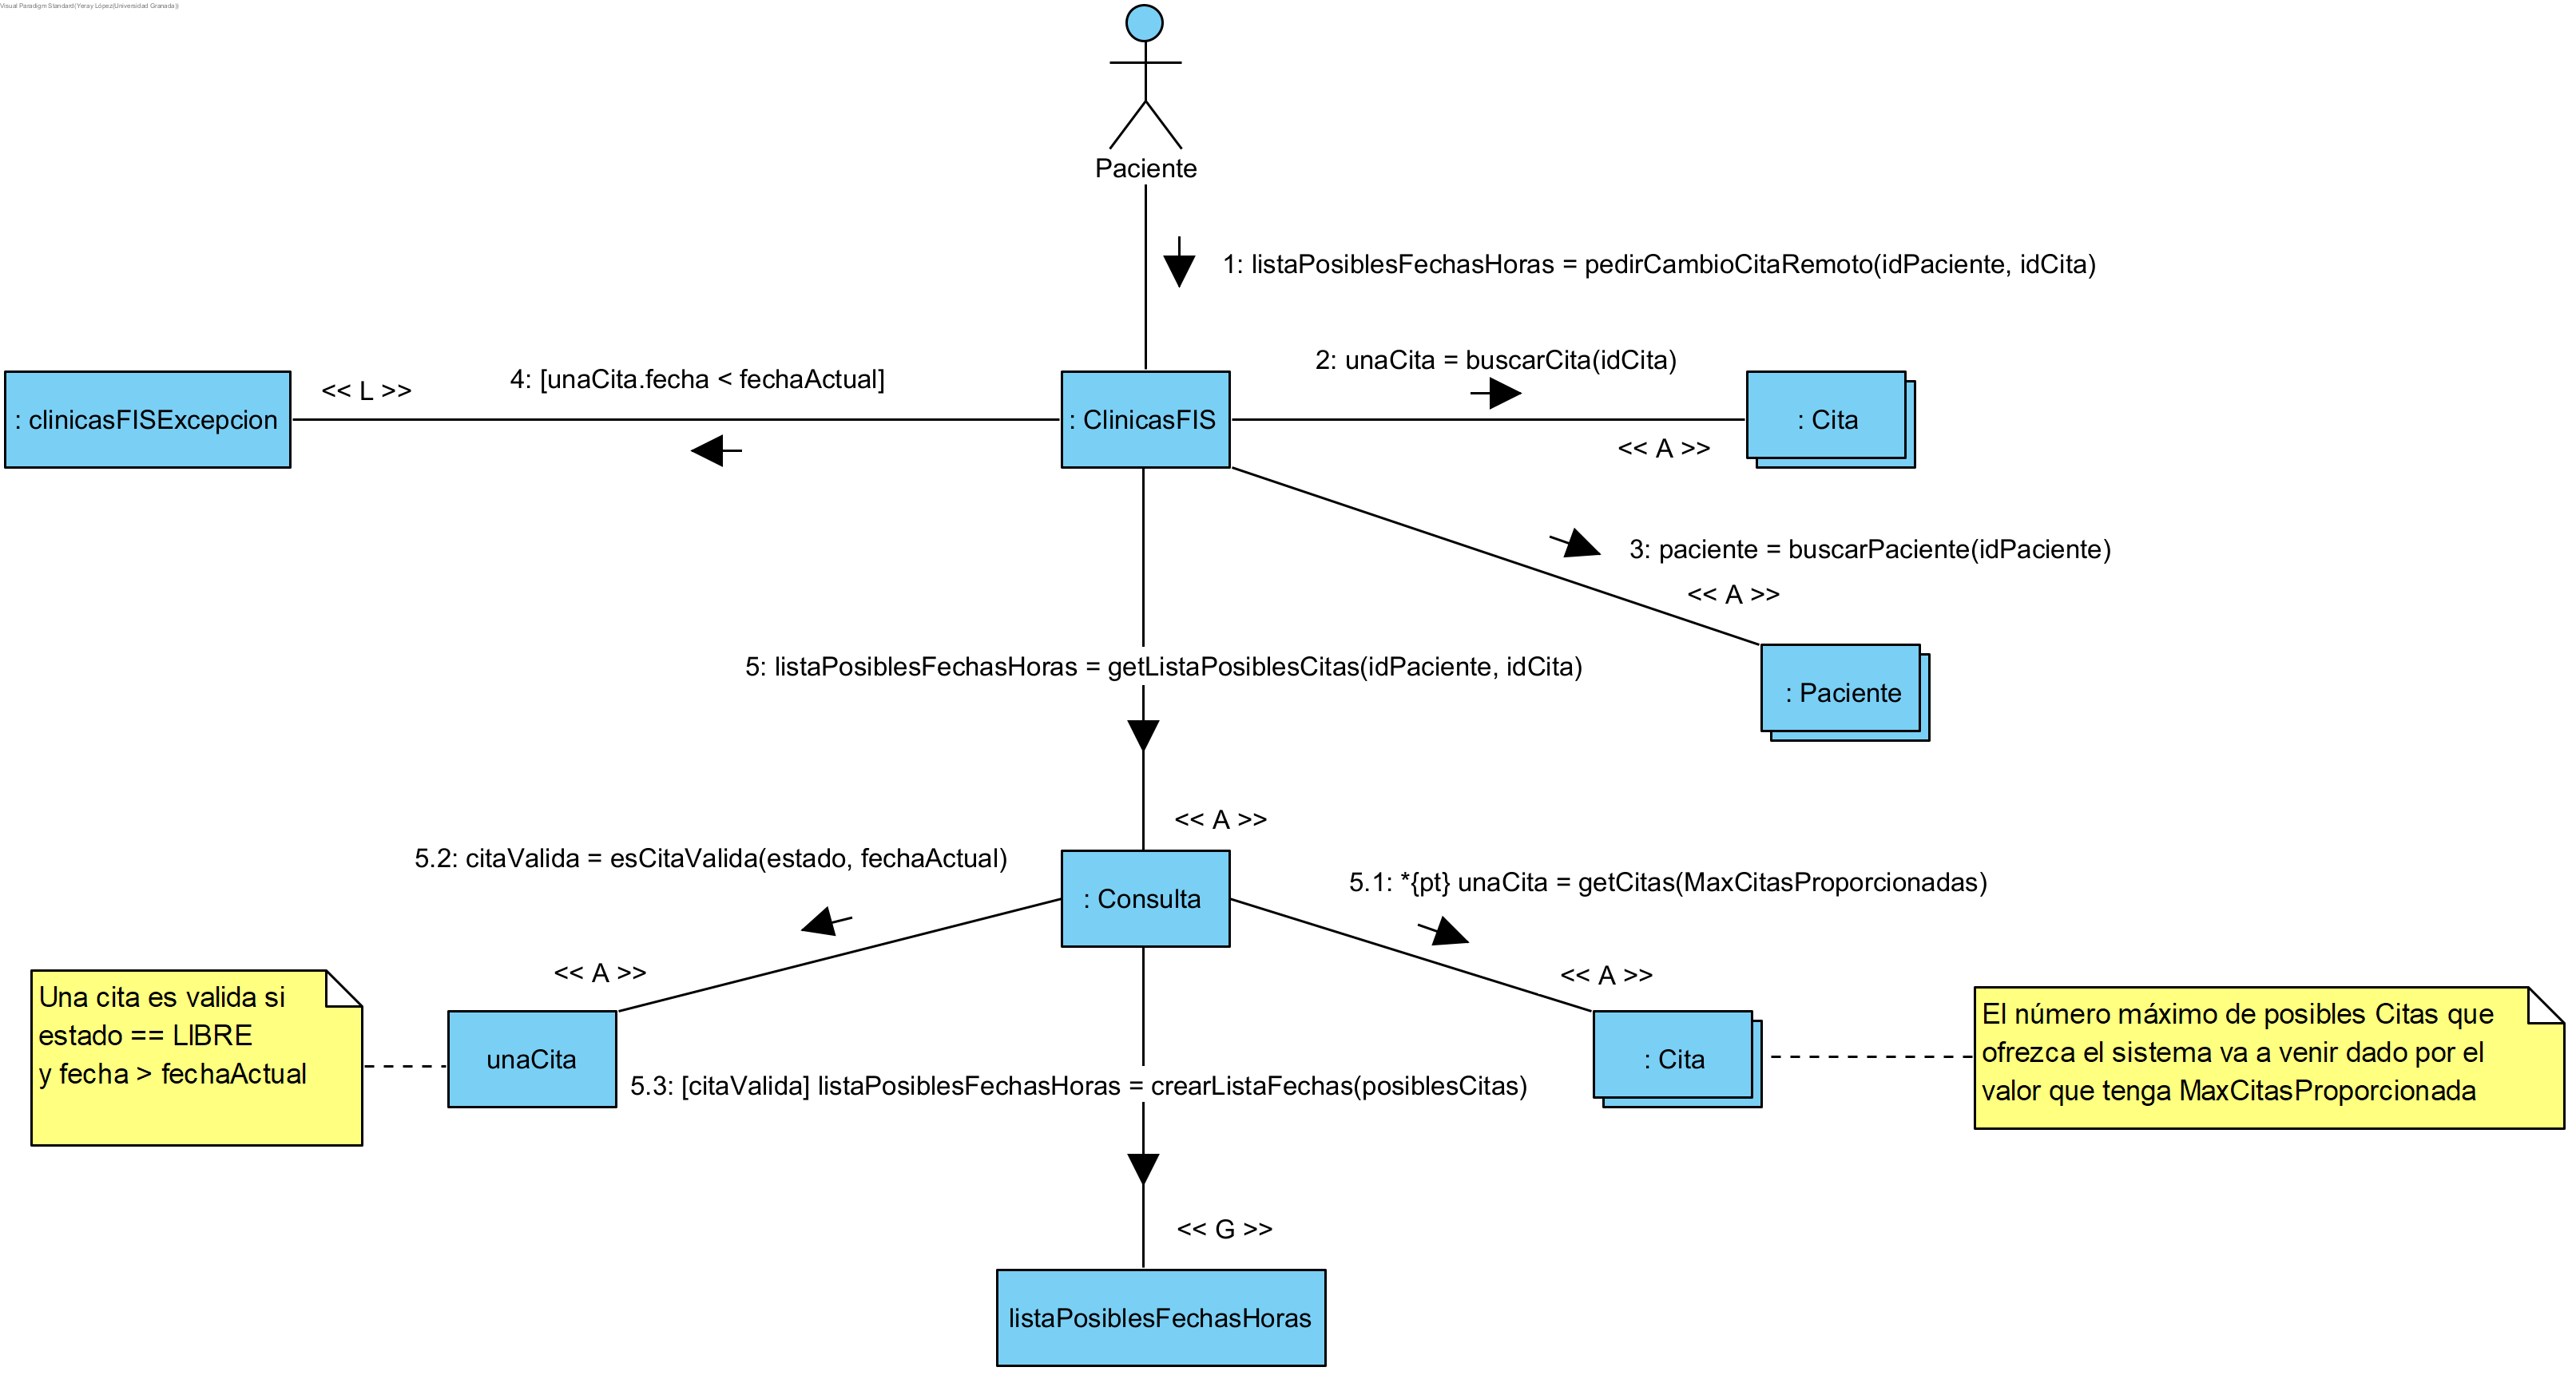
\includegraphics[scale = 0.40]{C18.png}\\[1.0 cm]\end{centering}
\begin{centering}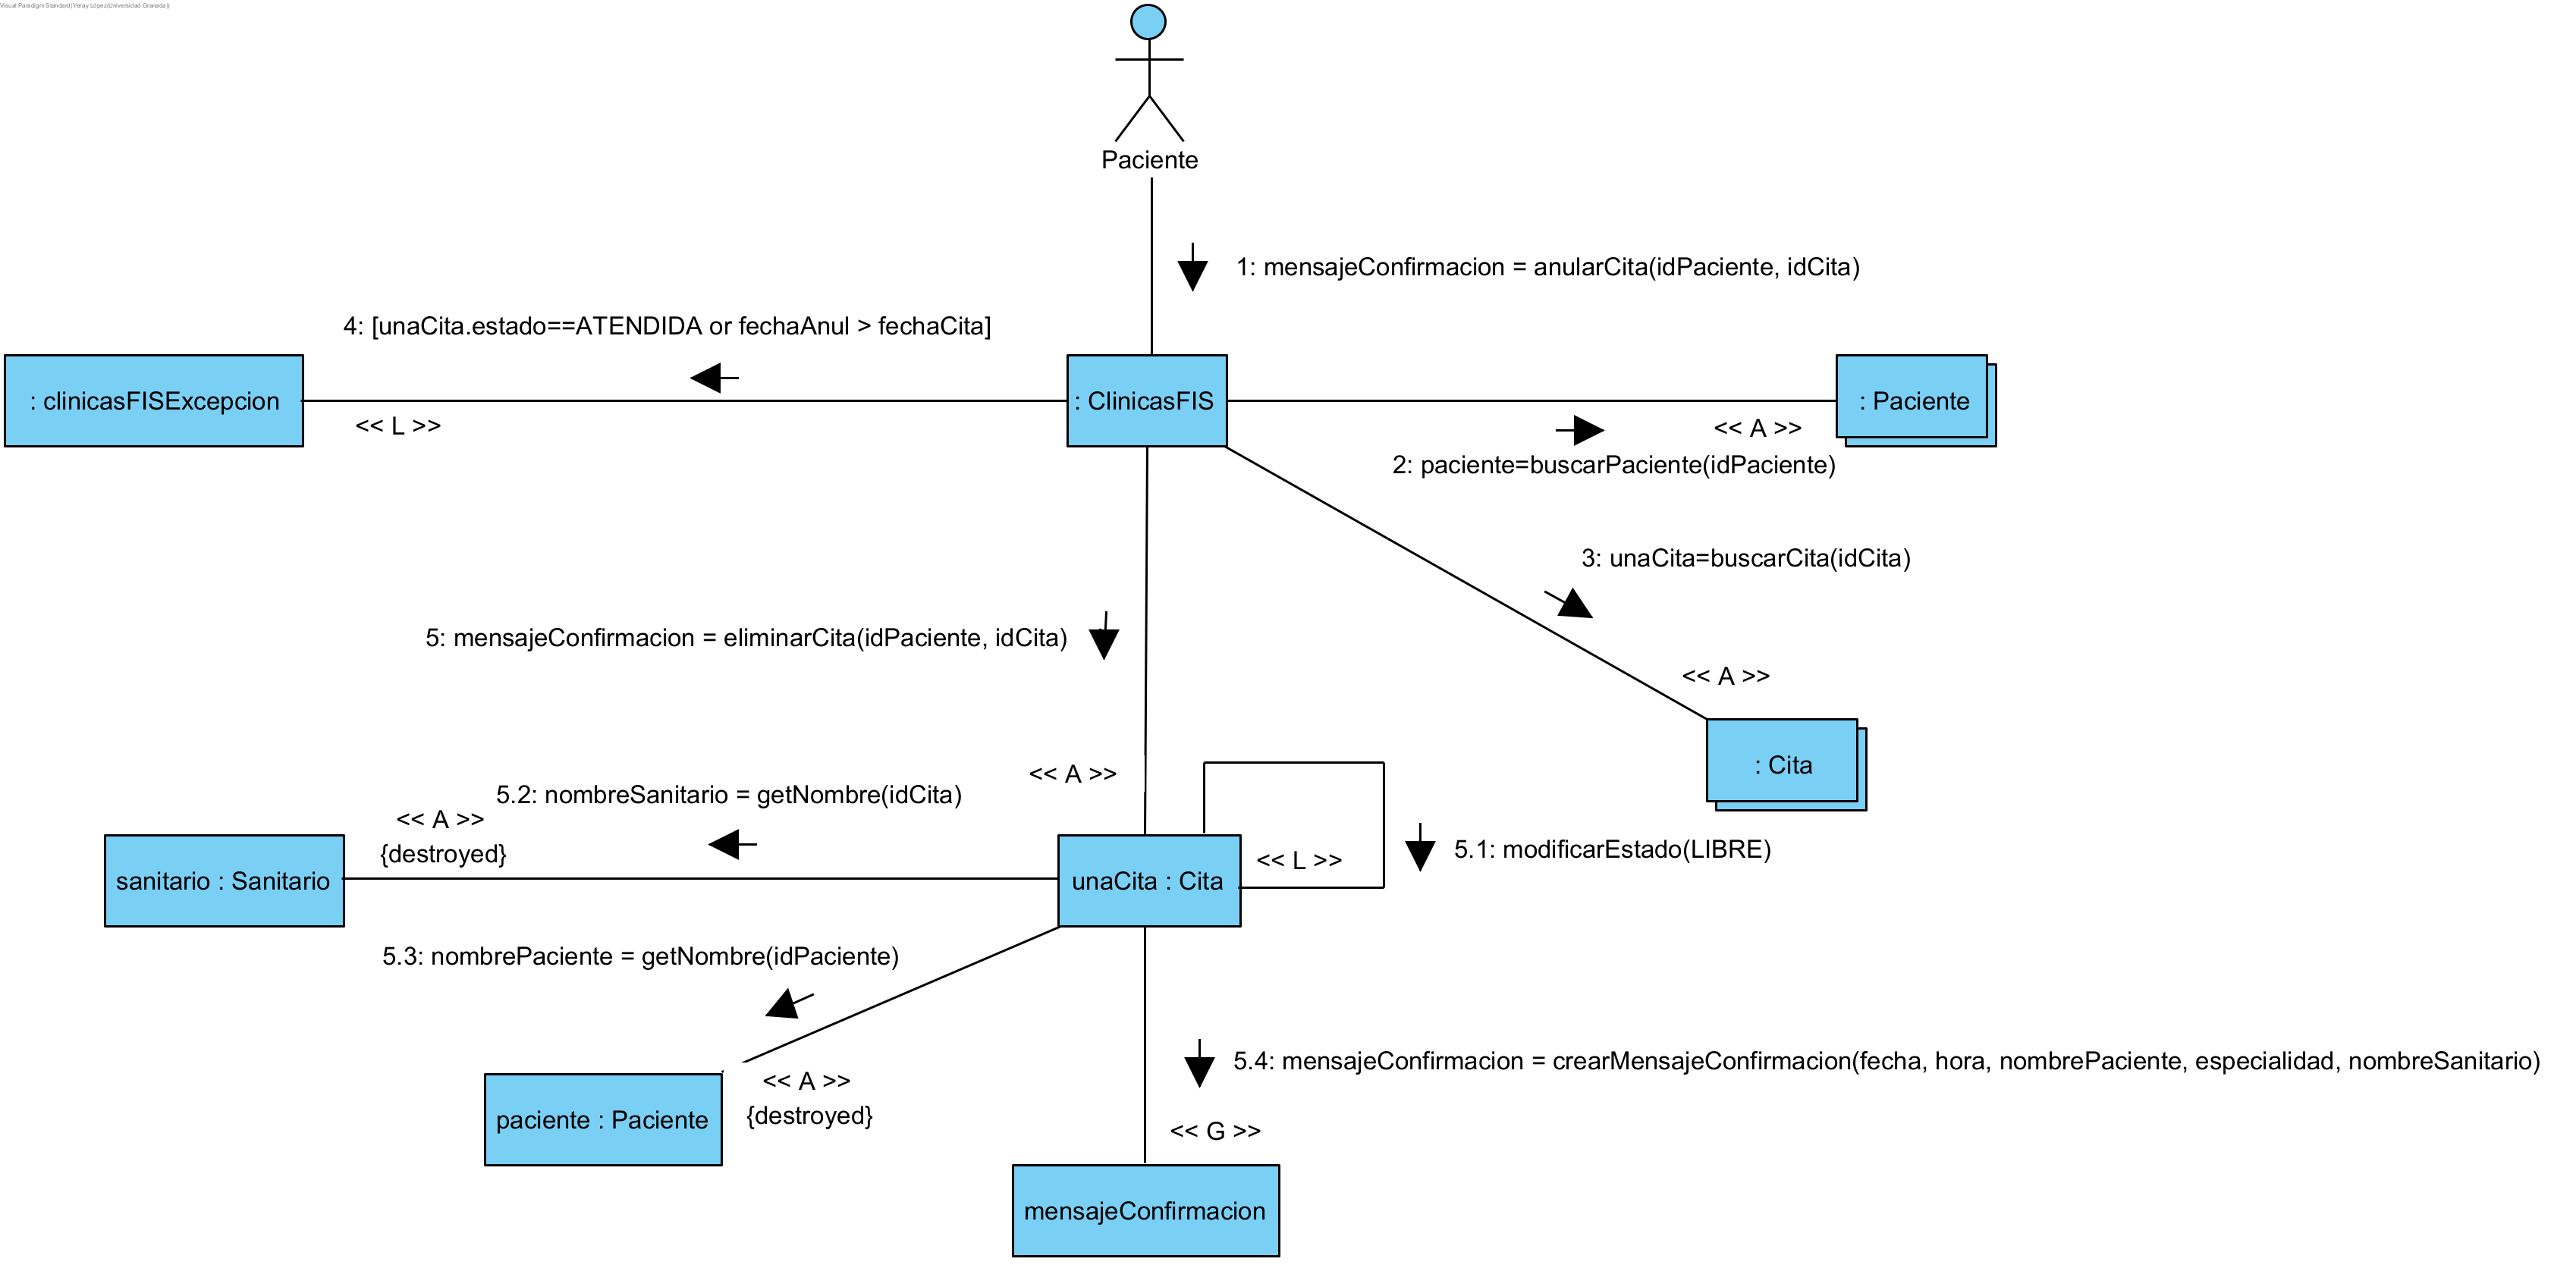
\includegraphics[scale = 0.40]{C19.png}\\[1.0 cm]\end{centering}
\begin{centering}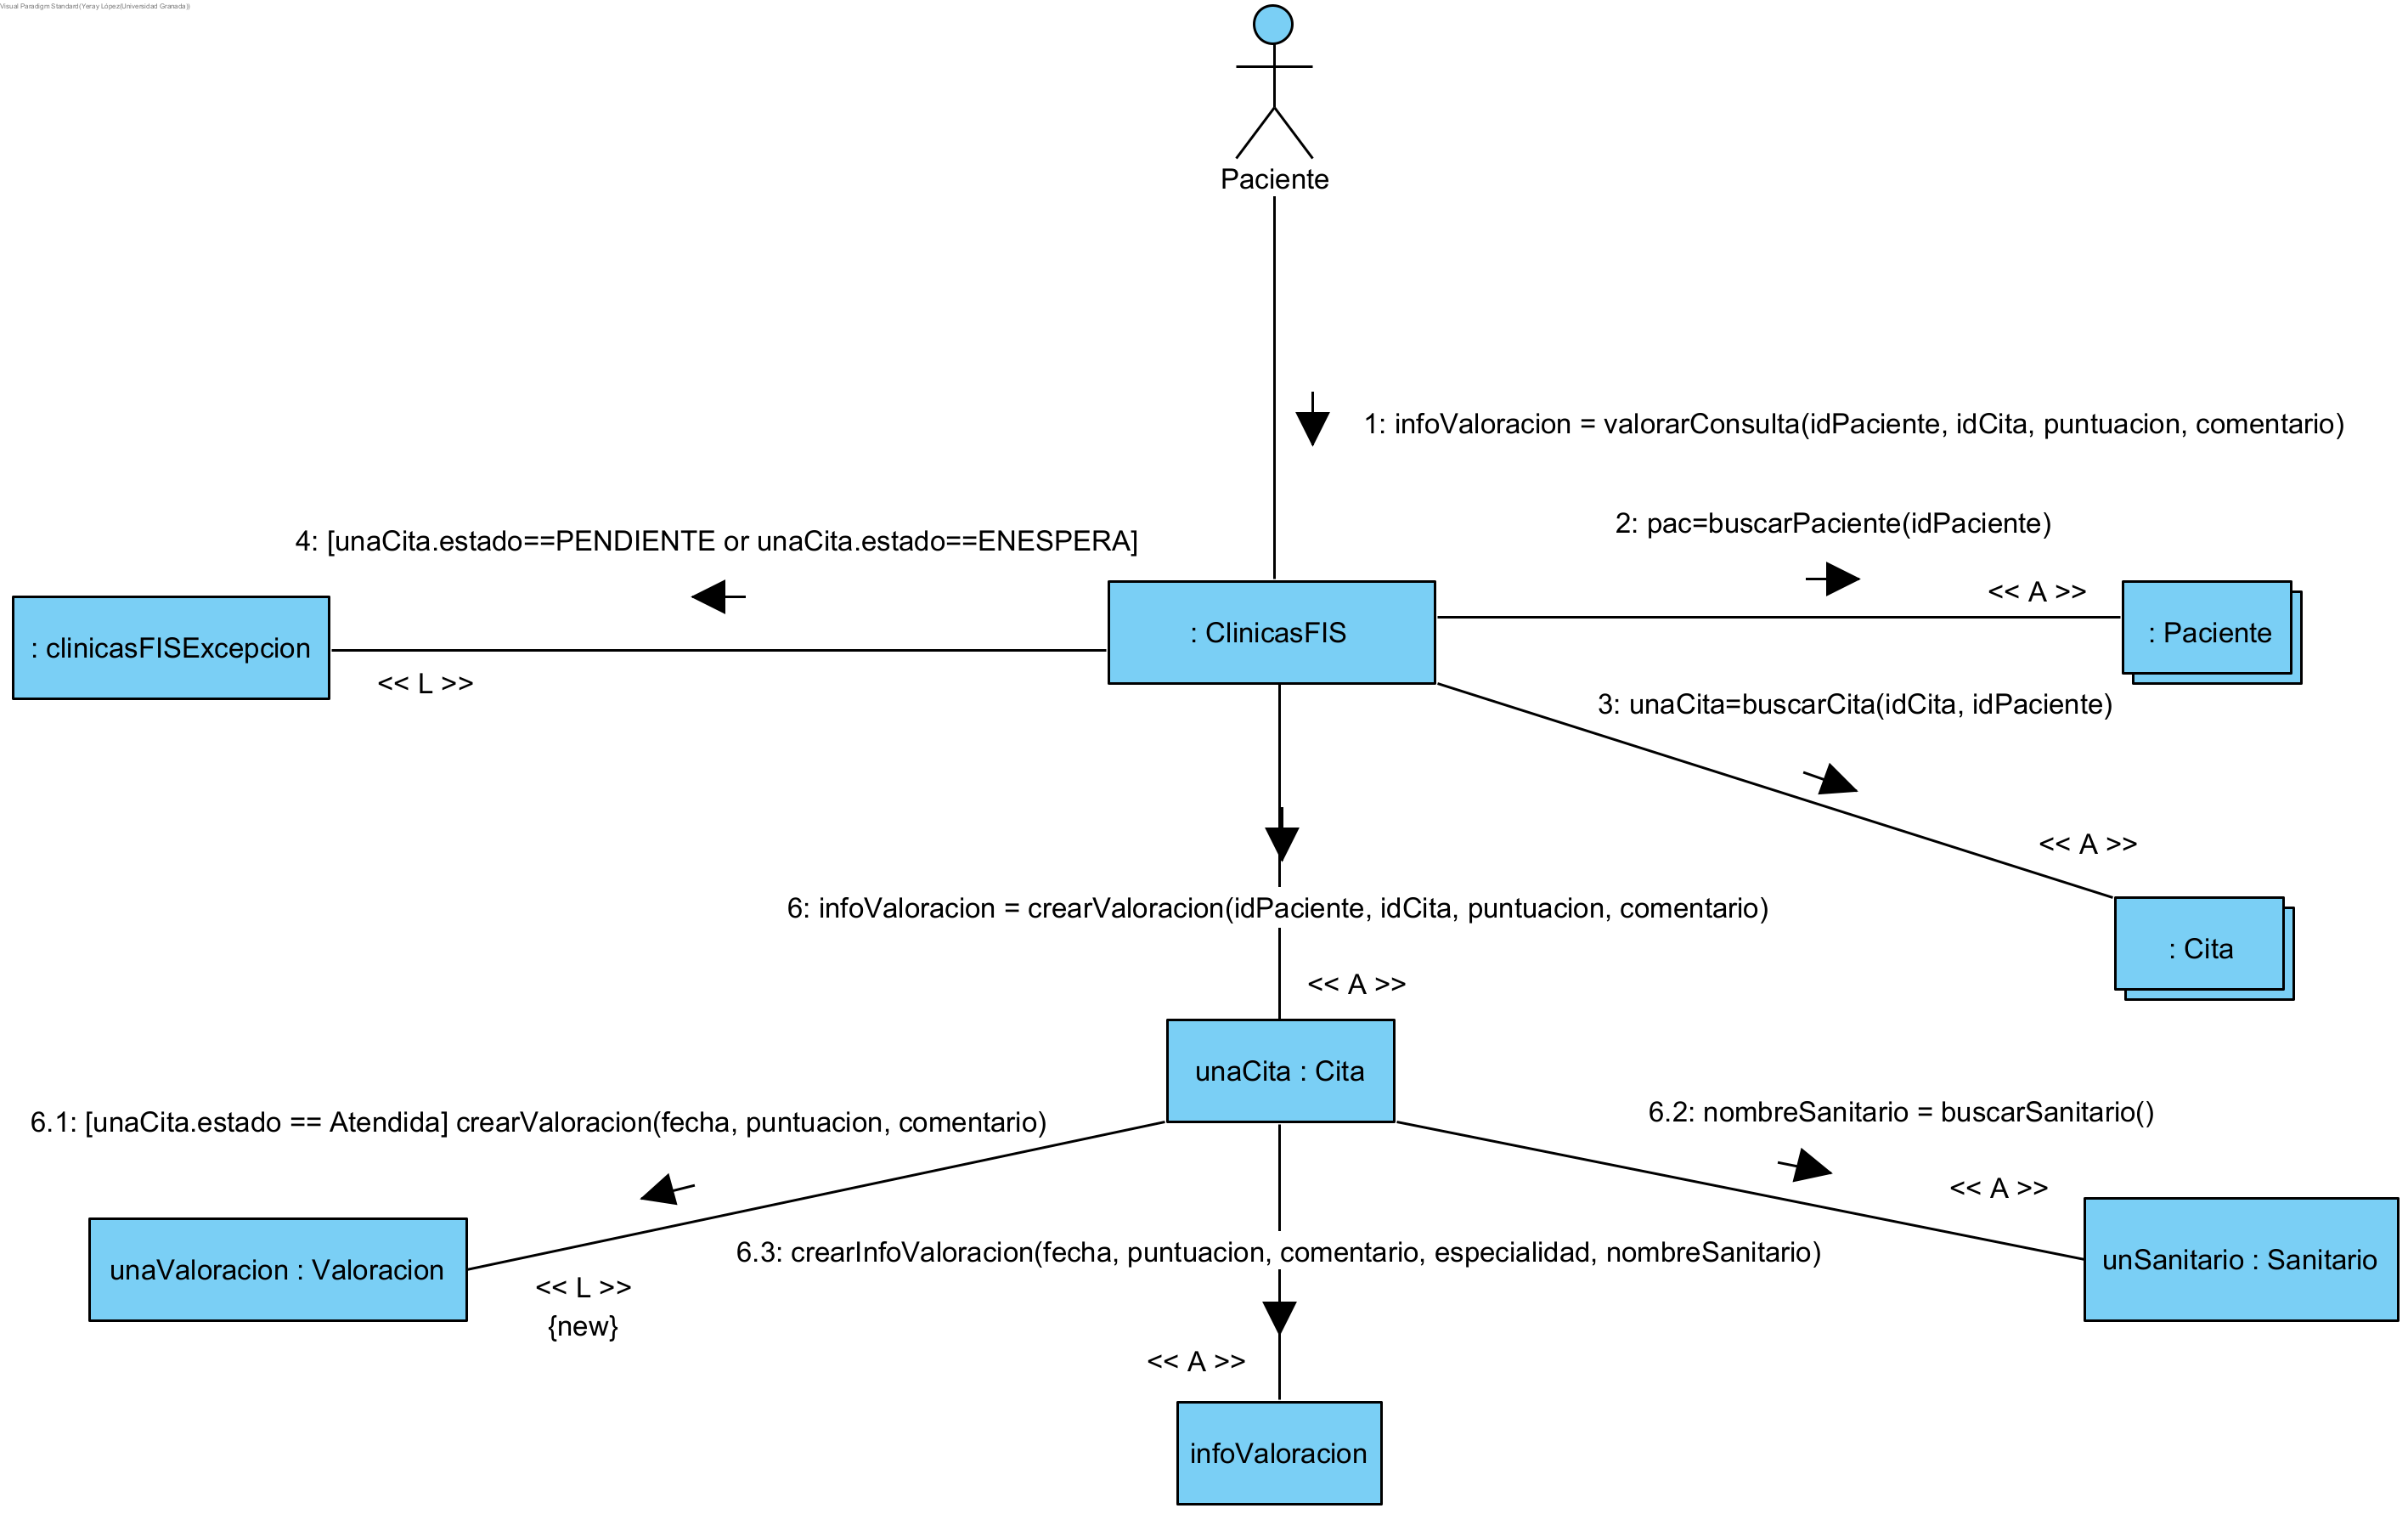
\includegraphics[scale = 0.50]{C20.png}\\[1.0 cm]\end{centering}

\pagebreak
\begin{landscape}
\thispagestyle{empty}
\section{Diagrama de clases}
Realizado por Martina Álvarez Lorenzo, Pablo Ariza García y Yeray López Ramirez.


\begin{centering}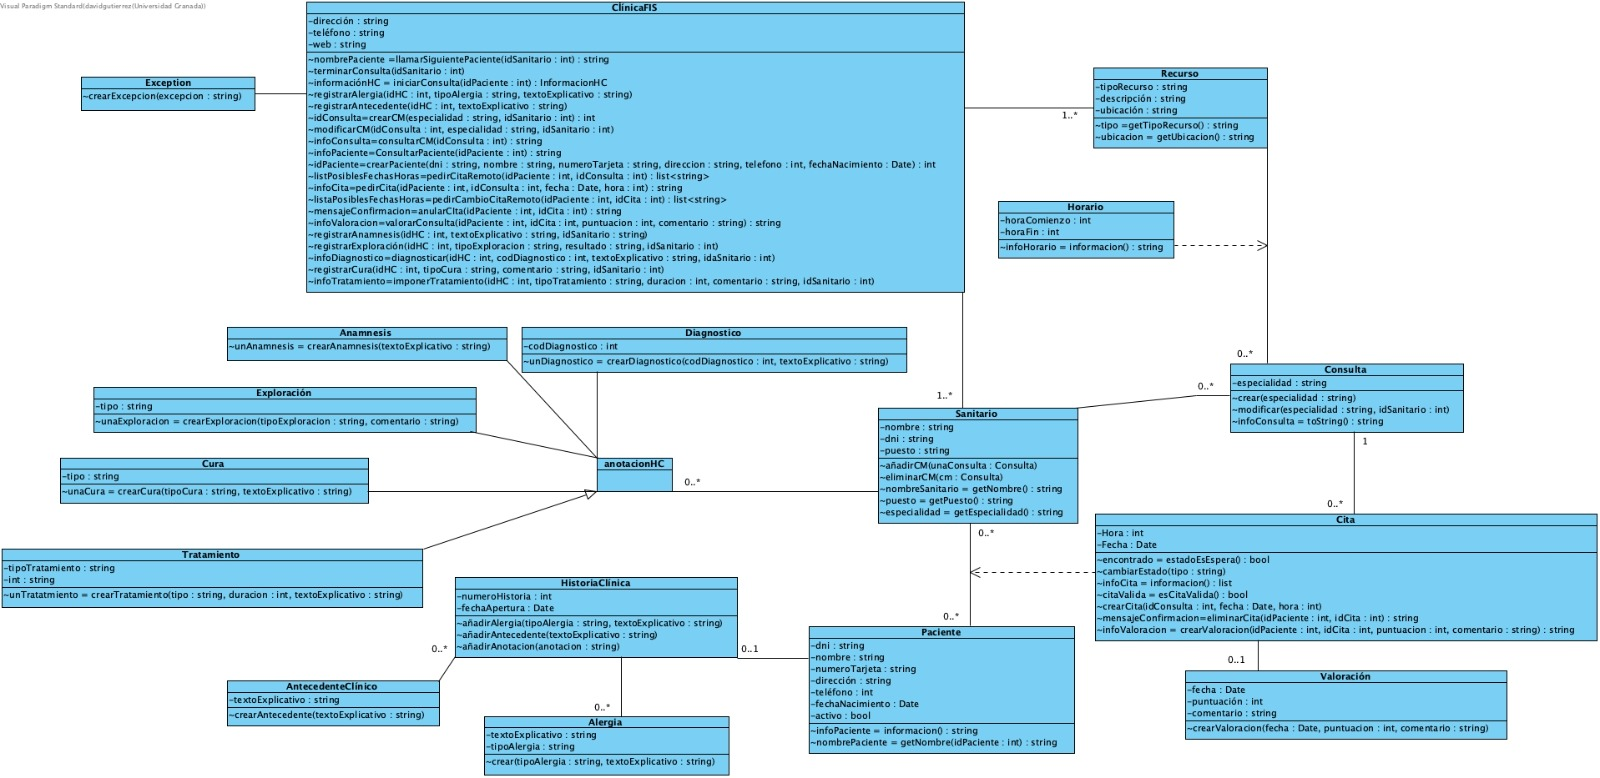
\includegraphics[scale = 0.45]{DiagramaDeClases.jpeg}\\[1.0 cm]\end{centering}

\vfill
\raisebox{12pt}{\makebox[\linewidth]{\thepage}}
\end{landscape}

\end{document}
